\documentclass[11pt,a4paper]{article}
\usepackage[margin=2cm]{geometry}
\usepackage[T1]{fontenc}
\usepackage[utf8]{inputenc}
\usepackage{lmodern,microtype}
\usepackage{amsmath,amssymb,mathtools,bm}
\usepackage{booktabs,tabularx,longtable,array,multirow}
\usepackage{graphicx,caption,subcaption,float}
\usepackage{enumitem,xcolor,hyperref,cleveref}
\usepackage[backend=biber,style=numeric-comp,sorting=none]{biblatex}
\addbibresource{references.bib}
\usepackage{fancyhdr,titlesec,siunitx,url}
\usepackage[most]{tcolorbox}
\usepackage{tikz}
\usetikzlibrary{arrows.meta,positioning,fit,calc,shapes.geometric,backgrounds}
\usepackage{listings}

\definecolor{deepblue}{RGB}{28,63,105}
\definecolor{deepgreen}{RGB}{38,105,79}
\definecolor{deeporange}{RGB}{170,92,20}
\definecolor{deepred}{RGB}{145,52,52}
\definecolor{softblue}{RGB}{232,241,250}
\definecolor{softgreen}{RGB}{235,247,240}
\definecolor{softorange}{RGB}{253,243,226}
\definecolor{softred}{RGB}{252,235,235}
\definecolor{softgray}{RGB}{245,246,248}
\hypersetup{colorlinks=true,linkcolor=deepblue,citecolor=deepgreen,urlcolor=deeporange,
 pdftitle={Geometry-MMALS G1 v1.1.0 Results and v1.1.1 Roadmap},pdfauthor={Guillaume Harbonnier}}
\pagestyle{fancy}\fancyhf{}\lhead{Geometry-MMALS G1}\rhead{v1.1.0 results and v1.1.1+ roadmap}\cfoot{\thepage}\setlength{\headheight}{14pt}
\titleformat{\section}{\Large\bfseries\color{deepblue}}{\thesection}{0.8em}{}
\titleformat{\subsection}{\large\bfseries\color{deepgreen}}{\thesubsection}{0.8em}{}
\titleformat{\subsubsection}{\normalsize\bfseries\color{deeporange}}{\thesubsubsection}{0.8em}{}
\setlist[itemize]{leftmargin=1.5em,itemsep=2pt,topsep=3pt}
\setlist[enumerate]{leftmargin=1.7em,itemsep=3pt,topsep=3pt}
\renewcommand{\arraystretch}{1.15}
\newcolumntype{Y}{>{\raggedright\arraybackslash}X}
\newcolumntype{C}{>{\centering\arraybackslash}X}
\newcommand{\MMALS}{\textsc{MMALS}}
\newcommand{\R}{\mathbb{R}}
\newcommand{\E}{\mathbb{E}}
\newcommand{\Pcal}{\mathcal{P}}
\newcommand{\loss}{\mathcal{L}}
\newcommand{\norm}[1]{\left\lVert #1 \right\rVert}
\newcommand{\softmax}{\operatorname{softmax}}
\newcommand{\relu}{\operatorname{ReLU}}
\newcommand{\KL}{\operatorname{KL}}
\newcommand{\diag}{\operatorname{diag}}
\newtcolorbox{plainbox}[1][]{title={#1},colback=softblue,colframe=deepblue!45,boxrule=.6pt,arc=2pt,left=8pt,right=8pt,top=7pt,bottom=7pt}
\newtcolorbox{positivebox}[1][]{title={#1},colback=softgreen,colframe=deepgreen!45,boxrule=.6pt,arc=2pt,left=8pt,right=8pt,top=7pt,bottom=7pt}
\newtcolorbox{warningbox}[1][]{title={#1},colback=softorange,colframe=deeporange!50,boxrule=.6pt,arc=2pt,left=8pt,right=8pt,top=7pt,bottom=7pt}
\newtcolorbox{criticalbox}[1][]{title={#1},colback=softred,colframe=deepred!50,boxrule=.6pt,arc=2pt,left=8pt,right=8pt,top=7pt,bottom=7pt}
\newtcolorbox{mathbox}[1][]{title={#1},colback=softgray,colframe=black!30,boxrule=.5pt,arc=1pt,left=8pt,right=8pt,top=7pt,bottom=7pt}

\begin{document}
\begin{titlepage}
\centering
\vspace*{0.6cm}
{\Huge\bfseries\color{deepblue} Geometry-MMALS G1 v1.1.0\par}
\vspace{0.25cm}
{\LARGE From Replicated Context Geometry\par}
\vspace{0.1cm}
{\LARGE to Partial Functional Routing\par}
\vspace{0.4cm}
{\Large Five-seed results, reviewer analysis, and the complete v1.1.1--v1.1.4 roadmap\par}
\vspace{0.7cm}
{\Large Guillaume Harbonnier\par}
\vspace{0.15cm}
{\normalsize Independent MMALS research program\par}
\vspace{0.15cm}
{\normalsize \href{https://github.com/gharbonnier78/geometry-mmalls-g1}{github.com/gharbonnier78/geometry-mmalls-g1}\par}
\vspace{0.55cm}
{\normalsize Evidence snapshot: RotatedMNIST, five matched-compute model seeds, June 2026\par}
\vfill
\begin{minipage}{0.94\textwidth}\small
\textbf{Epistemic status.} Version 1.1.0 is the first Geometry-MMALS experiment to freeze the replicated context geometry from v1.0.9 and compare three mechanisms that read the same map: a flexible MLP router, a 20-parameter linear router, and a 24-parameter prototype-energy router. The prototype improves nominal route order over the MLP on trained and held-out angles and improves functional optimal-transport route order on trained angles. That functional effect does not generalize to held-out angles. The linear router is at least as competitive and exhibits the strongest exploratory causal and ablation signals. Causal specificity, stable host ecology, memory transport, and operational superiority remain unqualified. The result therefore supports a partial representational-to-functional bridge, not a completed functional geometry.
\end{minipage}
\vfill
\end{titlepage}

\begin{abstract}
Geometry-MMALS asks whether a modular continual learner can acquire an internal context geometry, transmit it into routing decisions, allocate work to differentiated hosts, preserve those relations through continual updates, and eventually improve operational performance. Version 1.0.9 established replicated candidate evidence for the first step: a four-dimensional inferred context whose distances reflect rotation order and generalize to source identities not used to fit the decoder. Version 1.1.0 freezes that context and compares three matched-compute routers over five model seeds.

The prototype-energy router improves trained-factor nominal route distance-order correlation over the MLP by $0.088$ with 95\% seed interval $[0.035,0.142]$, and improves trained-factor functional optimal-transport route order by $0.046$ with interval $[0.004,0.089]$. Nominal route order also improves on the dense held-out angle grid by $0.038$ with interval $[0.013,0.064]$. In contrast, the held-out functional effect is only $0.007$ with interval $[-0.035,0.049]$. The low-capacity linear router reaches the highest mean route correlations and the strongest exploratory causal and ablation signals, while the prototype creates sharper route territories but fails the preregistered causal-specificity, identity-preservation, and host-ecology gates. Accuracy and forgetting remain operationally equivalent rather than superior.

The article explains the experiment in accessible language and then formalizes the router as an operator $R_\theta:\Pcal(Z\times M)\to\Pcal(H)$. It incorporates a versioned reviewer and verification interpretation, specifies v1.1.1 as a local-stability and bridge-isolation experiment using a common frozen host bank and common functional cost matrix, and defines the subsequent v1.1.2 SPD covariance, v1.1.3 route-function memory, v1.1.4 causal specialization, G2 energy-guided control, and mandatory verification-stack stages. No Riemannian-manifold, operational-superiority, memory-transport, or quantum-advantage claim is made.
\end{abstract}
\tableofcontents
\clearpage

\section{The scientific path in plain language}
\begin{plainbox}[What the program constructs]
Imagine training a system to recognize handwritten digits rotated to $-60^\circ$, $-30^\circ$, $0^\circ$, $30^\circ$, and $60^\circ$. The system sees these conditions progressively, one continual-learning stage at a time.

Inside the system:
\begin{itemize}
\item $z_0$ is the frozen sensory view of the image;
\item $c\in\R^4$ is the inferred context, a four-number description of the current situation;
\item $r\in\Delta^{H-1}$ is the route, a probability distribution assigning work to $H$ hosts;
\item $g_h$ are small specialist transformations;
\item $z_M=\sum_h r_h g_h(z_0)$ is the routed synthesis used for classification.
\end{itemize}
\end{plainbox}

\subsection{What was already known after v1.0.9}
The context space had become a useful map. Nearby rotation angles tended to occupy nearby context positions, and unseen source identities still carried decodable angle information. This was the first replicated representational result of the program.

The unresolved problem was downstream use. A route can be numerically computed from a context without preserving its geometry. A flexible router may exploit information while folding, stretching, or discarding the metric relations that made the context scientifically interesting.

\subsection{The employee-and-map analogy, updated}
In v1.0.9, the employee had a good map but did not demonstrate that the map organized the dispatch process. In v1.1.0, three employees receive exactly the same map:
\begin{itemize}
\item one can use a large flexible rulebook (MLP);
\item one can use only a simple linear rule (linear router);
\item one sends work toward host territories represented by learned centers (prototype-energy router).
\end{itemize}
The simple and prototype-based employees organize dispatch more consistently with the map than the flexible employee. However, the departments receiving the work are not yet reliably different in function, and the dispatch system is not yet better at its operational job.

\subsection{Three evidence levels}
\begin{enumerate}
\item \textbf{Representational:} the context reflects the external factor. Achieved as replicated candidate evidence in v1.0.9.
\item \textbf{Functional:} ordered context changes cause ordered and meaningful host allocation. v1.1.0 reaches only a partial structural form of this level.
\item \textbf{Operational:} the chain improves accuracy, retention, robustness, cost, or another declared objective. Not reached.
\end{enumerate}

\begin{positivebox}[Why v1.1.0 is still an advance]
Before this experiment, it was unknown whether the context geometry could be transmitted at all. The five-seed result shows that low-capacity routing can preserve more of the context order than a flexible MLP. The remaining failure is now narrower: the system must connect route movement to stable differences in host function and make that connection generalize beyond trained factor values.
\end{positivebox}

\section{Formal operator view}
\subsection{The reusable branch definition}
The broader Geometry-MMALS branch treats routing as an operator between distributions of representations and memories and distributions over hosts:
\begin{equation}
R_\theta:\Pcal(Z\times M)\longrightarrow\Pcal(H)\cong\Delta^{K-1}.
\end{equation}
An empirical state at time $t$ can be written
\begin{equation}
\mu_t=\frac1N\sum_{j=1}^{N}\delta_{(z_j,m_j)},
\qquad
\pi_H=R_\theta(\mu_t).
\end{equation}
The geometry branch asks whether this operator is locally continuous, stable under perturbation, coherent with the functions implemented by the hosts, and reproducible across seeds.

\subsection{The controlled v1.1.0 special case}
In the executed protocol, memory is fixed or omitted and the router reads the normalized four-dimensional context:
\begin{equation}
R_\theta:\mathbb S^3\longrightarrow\Delta^{H-1}.
\end{equation}
This restricted setting isolates the context-to-route bridge before adding memory, goals, host-state feedback, or future-control terms.

\subsection{Boundary with TPUT}
Goal-conditioned routing belongs primarily to TPUT:
\begin{equation}
R_\theta:\Pcal(Z\times M)\times G\longrightarrow\Pcal(H).
\end{equation}
Geometry-MMALS may compare a family $\{R_\theta^{(g)}\}_{g\in G}$, but it should not duplicate the RL or forward--backward controller. The geometric route energy developed here is a component that TPUT can later condition on objectives and futures.

\subsection{No manifold assumption by default}
The program does not assume that the latent space is Riemannian. Intrinsic distance, tangent spaces, exponential/logarithmic maps, Karcher means, or SPD geometry may be tested as methodological candidates, but they are retained only when they improve prediction, stability, drift detection, specialization, compactness, or auditability. This follows a test-first rather than elegance-first interpretation of geometric deep learning \cite{bronstein2021geometric,amari1998natural}.

\section{Executed v1.1.0 protocol}
\subsection{Matched treatments}
For each model seed, the v1.0.9 aligned context checkpoint is reproduced, hashed, and frozen. A common host, synthesis-normalization, and classifier state is then copied into three treatments:
\begin{align}
R_0(c)&=\softmax\!\left(W_2\phi(W_1c+b_1)+b_2\right),\\
R_1(c)&=\softmax(Wc+b),\\
E_h^{\mathrm{geo}}(c)&=\frac{d_C(c,\mu_h)^2}{2\sigma_h^2}+b_h,\\
R_{2,h}(c)&=\frac{\exp[-E_h^{\mathrm{geo}}(c)/\tau]}{\sum_k\exp[-E_k^{\mathrm{geo}}(c)/\tau]},
\end{align}
where $d_C(a,b)=\tfrac12\norm{a-b}_2$ on the normalized context sphere.

The MLP has 4,740 parameters, the linear router 20, and the prototype-energy router 24. All methods receive the same 15,360 forward images and 80 optimizer steps per seed.

\subsection{Primary routing loss}
The routing phase contains no angle-supervised route-geometry term:
\begin{equation}
\loss=\loss_{\mathrm{CE}}+\lambda_A\loss_{\mathrm{anchor}}+\lambda_B\loss_{\mathrm{balance}}+\lambda_D\loss_{\mathrm{host-div}}.
\end{equation}
Therefore, any greater preservation of factor order arises from architecture and learned task behavior rather than direct angle supervision during router training.

\subsection{Nominal route geometry}
Historical route geometry uses the normalized root-simplex chord
\begin{equation}
d_R(r_a,r_b)=\frac{\norm{\sqrt{r_a}-\sqrt{r_b}}_2}{\sqrt2}.
\end{equation}
This is related to Hellinger/Fisher--Rao geometry but treats host coordinates as fixed and semantically independent.

\subsection{Functional route geometry}
Two route vectors can differ numerically while assigning mass between functionally similar hosts. A host cost matrix is therefore estimated:
\begin{equation}
C_{hk}=\E_x\left[\frac{\norm{g_h(z_0(x))-g_k(z_0(x))}_2^2}{d_M}\right].
\end{equation}
Route displacement is evaluated by entropic optimal transport \cite{peyre2019ot,cuturi2013sinkhorn}:
\begin{equation}
W_C^\varepsilon(r_a,r_b)=
\min_{\Pi\ge0}\langle\Pi,C\rangle+
\varepsilon\KL\!\left(\Pi\middle\|r_ar_b^\top\right),
\quad
\Pi\mathbf 1=r_a,\;\Pi^\top\mathbf 1=r_b.
\end{equation}

\subsection{Disjoint evidence partitions}
Five disjoint source-identity partitions are used for host-cost construction, mediation-probe fitting, mediation-probe evaluation, tangent fitting, and final causal/ablation evaluation. The source identity, not the pairwise distance, is the within-seed bootstrap unit. The model seed is the replication unit.

\section{Results}
\subsection{Protocol integrity}
\begin{positivebox}[C0 passes]
The frozen context is numerically identical across all routing treatments: the maximum absolute context difference is zero. Every method in every seed uses 15,360 forward images and 80 optimizer steps. Five seeds complete without runtime source patching.
\end{positivebox}

\subsection{Route geometry by method}
\begin{figure}[H]\centering
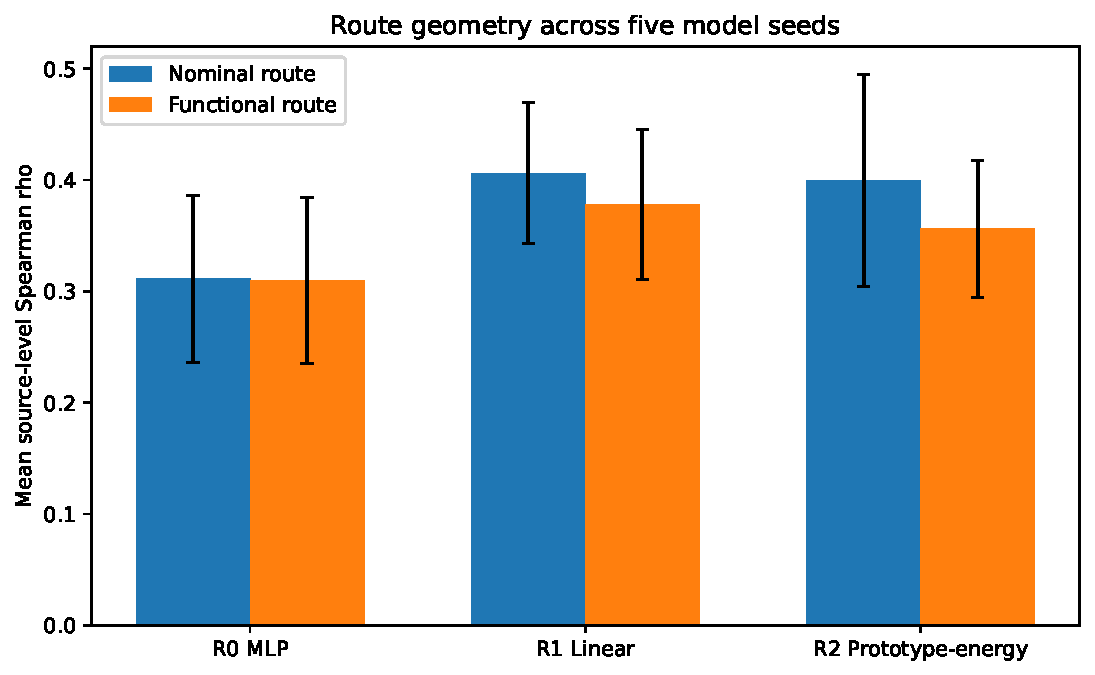
\includegraphics[width=.82\textwidth]{figures/route_geometry_summary.pdf}
\caption{Mean source-level route distance-order correlation across five seeds. Error bars are 95\% Student-$t$ intervals over model seeds.}
\end{figure}

\begin{table}[H]\centering\small
\caption{Five-seed method summaries.}
\begin{tabular}{lccccc}
\toprule
Method & Nominal $\rho$ & Functional $\rho$ & Held-out acc. & Final train acc. & Forgetting\\
\midrule
R0 MLP & 0.311 & 0.310 & 0.5692 & 0.6303 & 0.0979\\
R1 Linear & \textbf{0.406} & \textbf{0.378} & 0.5658 & \textbf{0.6284} & 0.1012\\
R2 Prototype-energy & 0.400 & 0.356 & 0.5668 & 0.6280 & \textbf{0.0929}\\
\bottomrule
\end{tabular}
\end{table}

The principal R2--R0 effects are shown in \cref{fig:primaryeffects}.
\begin{figure}[H]\centering
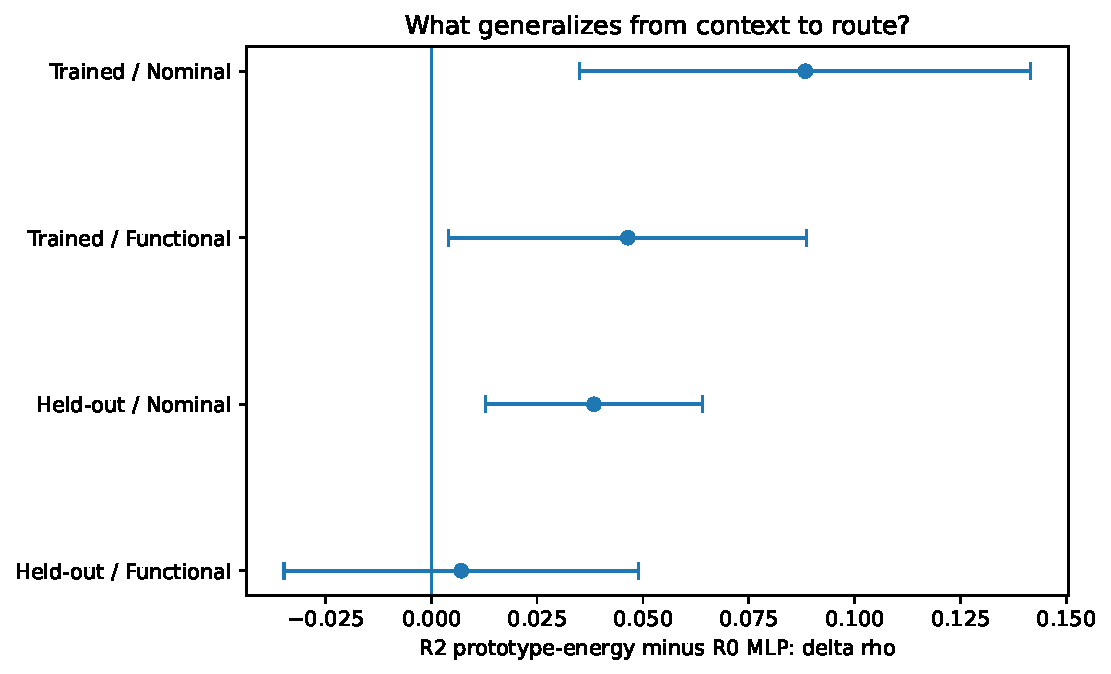
\includegraphics[width=.82\textwidth]{figures/primary_route_effects.pdf}
\caption{Prototype-energy minus MLP route-order effects. The trained nominal and trained functional intervals exclude zero; the held-out nominal interval excludes zero; the held-out functional interval does not.}\label{fig:primaryeffects}
\end{figure}

\subsection{What the prototype demonstrates}
On trained factors,
\begin{align}
\Delta\rho_{\mathrm{nominal}}&=+0.088, &95\%\ \mathrm{CI}&=[+0.035,+0.142],\\
\Delta\rho_{\mathrm{functional}}&=+0.046, &95\%\ \mathrm{CI}&=[+0.004,+0.089].
\end{align}
All five seeds favor the prototype in both cases. On the dense held-out grid,
\begin{align}
\Delta\rho_{\mathrm{nominal,heldout}}&=+0.038, &95\%\ \mathrm{CI}&=[+0.013,+0.064],\\
\Delta\rho_{\mathrm{functional,heldout}}&=+0.007, &95\%\ \mathrm{CI}&=[-0.035,+0.049].
\end{align}

\begin{warningbox}[Central qualification]
Nominal route order generalizes to unseen factor values. Functional route order is observed on trained factors but is not established on held-out factors. A reviewer-safe statement must keep these claims separate.
\end{warningbox}

\subsection{The linear-router surprise}
The linear router reaches the highest mean nominal and functional correlations with only 20 parameters. Its trained nominal effect over the MLP is $+0.095$ with interval $[+0.009,+0.181]$. The prototype does not outperform the linear router on either route metric.

This suggests that the relevant factor direction may be globally transmitted by a simple affine map, whereas the prototype architecture forms local territories. On a curved context arc, local prototype activations can create sharp neighborhoods without preserving a single monotonic global direction.

\subsection{Mediation probes}
\begin{figure}[H]\centering
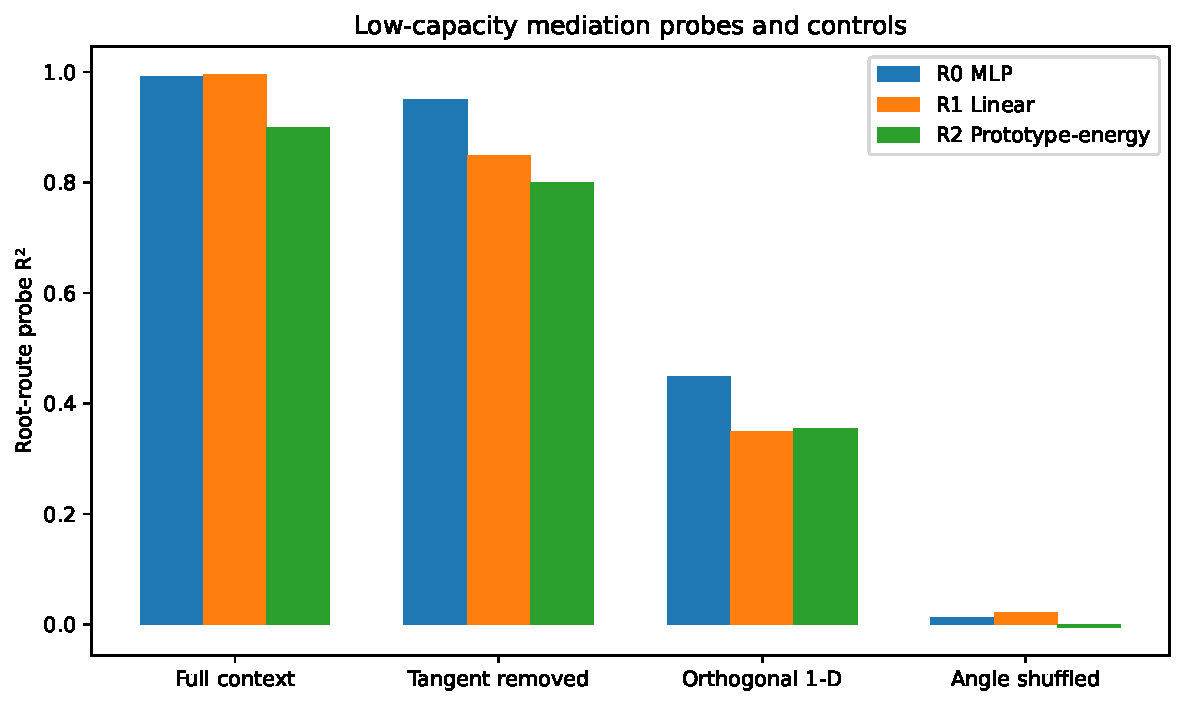
\includegraphics[width=.86\textwidth]{figures/probe_controls.pdf}
\caption{Low-capacity context-to-root-route probes. Full-context reconstruction is high for all methods, but factor shuffling destroys it. Removing the fitted tangent harms the linear and prototype routers more than the MLP.}
\end{figure}
A high probe score alone is not causal evidence because the route is computed from context by construction. The controls are the informative part. Removing the factor tangent reduces route reconstruction most strongly for the linear router, indicating that its simple mapping relies more directly on the factor-relevant component.

\subsection{Causal specificity}
\begin{figure}[H]\centering
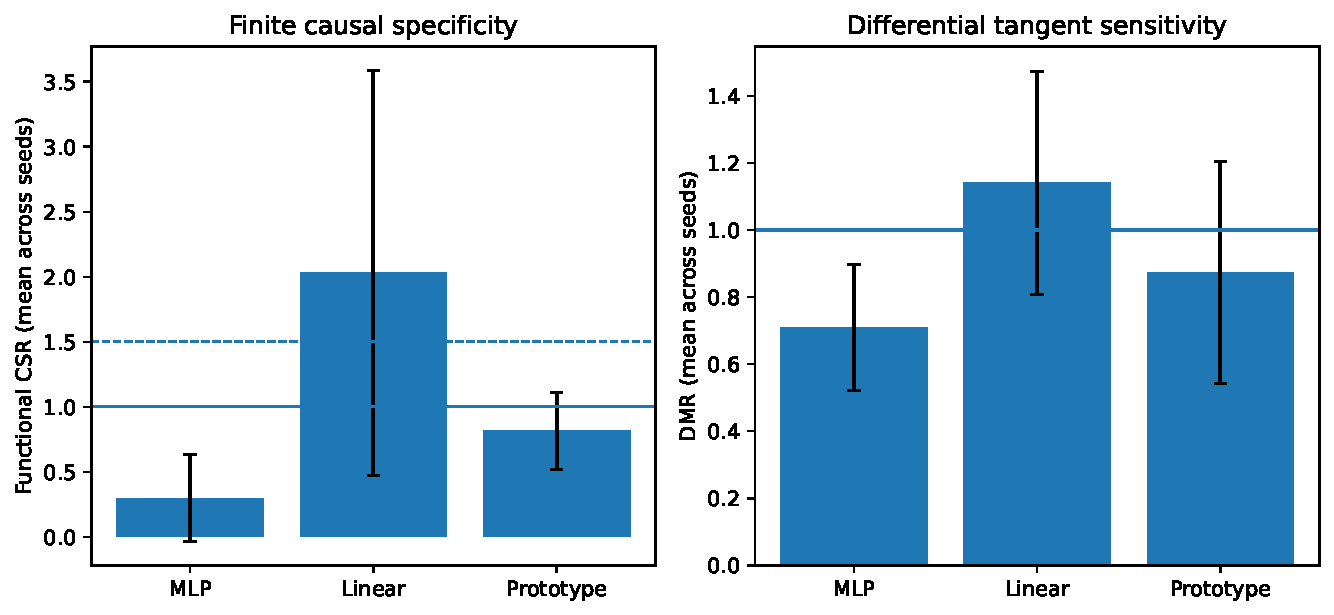
\includegraphics[width=.9\textwidth]{figures/causal_summary.pdf}
\caption{Finite functional causal-specificity ratio (CSR) and differential mediation ratio (DMR). Dashed CSR line marks the preregistered candidate threshold of 1.5; the solid line marks tangent/orthogonal parity.}
\end{figure}
The prototype mean functional CSR is 0.814 and mean DMR 0.873. It fails the causal-specificity gate and fails prediction-identity preservation in the required fraction of seeds. The linear router has the strongest exploratory functional CSR (mean 2.03), but only two of five seeds achieve a source-bootstrap lower bound above one. Thus it is a strong lead, not a passed claim.

\subsection{Host ecology}
\begin{figure}[H]\centering
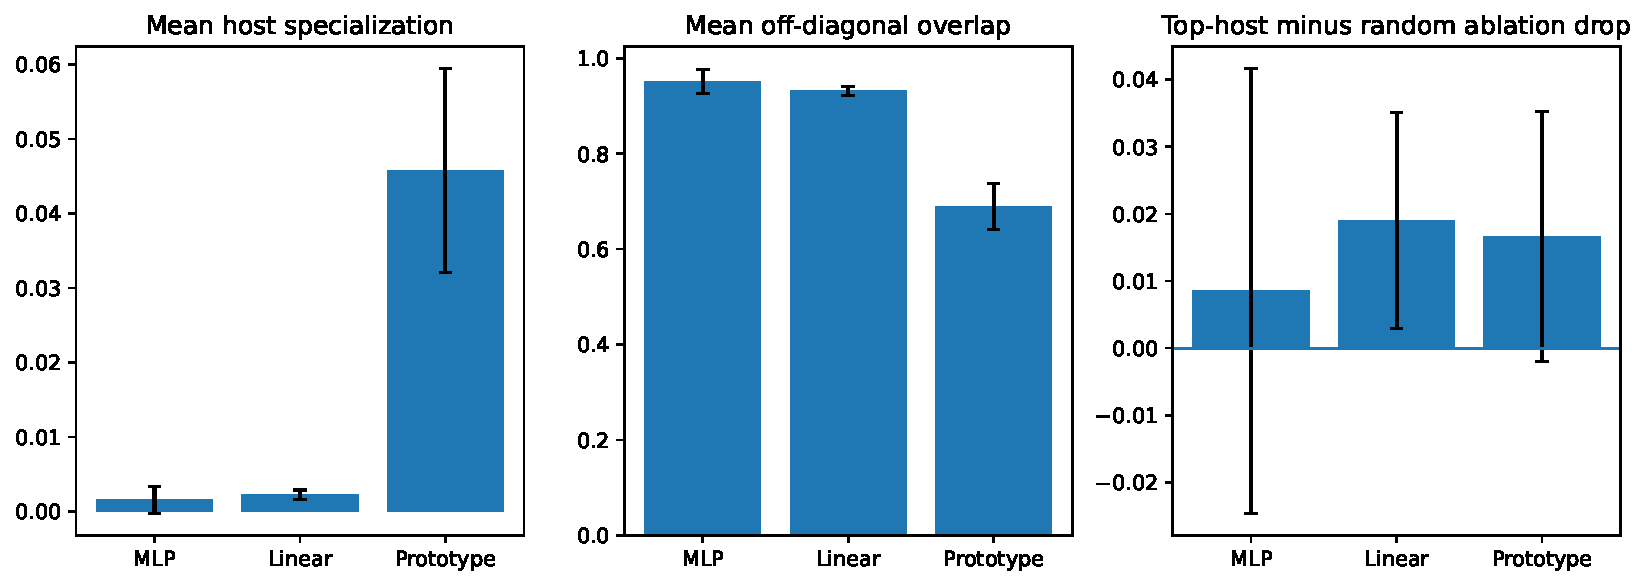
\includegraphics[width=.98\textwidth]{figures/host_ecology_summary.pdf}
\caption{Host ecology summaries. Prototype routing creates sharper territories and lower overlap, but top-host ablation is not reproducibly stronger than a deterministic random-host control.}
\end{figure}
\begin{figure}[H]\centering
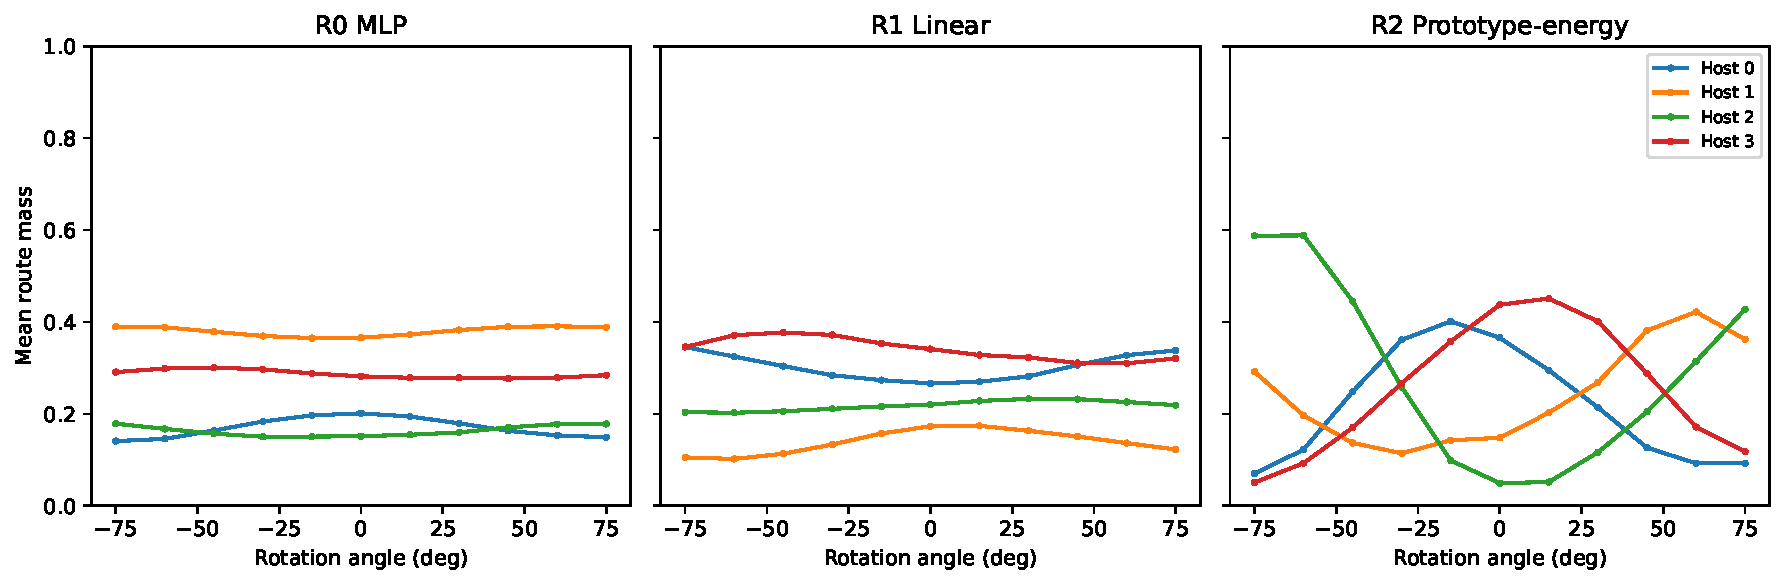
\includegraphics[width=.98\textwidth]{figures/host_territories_seed0.pdf}
\caption{Illustrative seed-0 host territories across the dense angle grid. These plots visualize routing structure but do not by themselves establish functional specialization.}
\end{figure}
The prototype has the greatest route-mass specialization and the lowest territory overlap. However, only three of five seeds show a larger mean accuracy drop for removal of the top-routed host than for removal of the random control host. The linear router shows this sign in all five seeds and has the largest mean excess ablation drop.

\begin{plainbox}[Territories are not yet competencies]
A routing territory says where an expert receives work. A functional specialization claim additionally requires that the expert performs a distinct and reproducible function, and that its removal or route swap causes a localized effect. v1.1.0 observes territories but does not qualify mature host ecology.
\end{plainbox}

\subsection{Operational metrics}
\begin{figure}[H]\centering
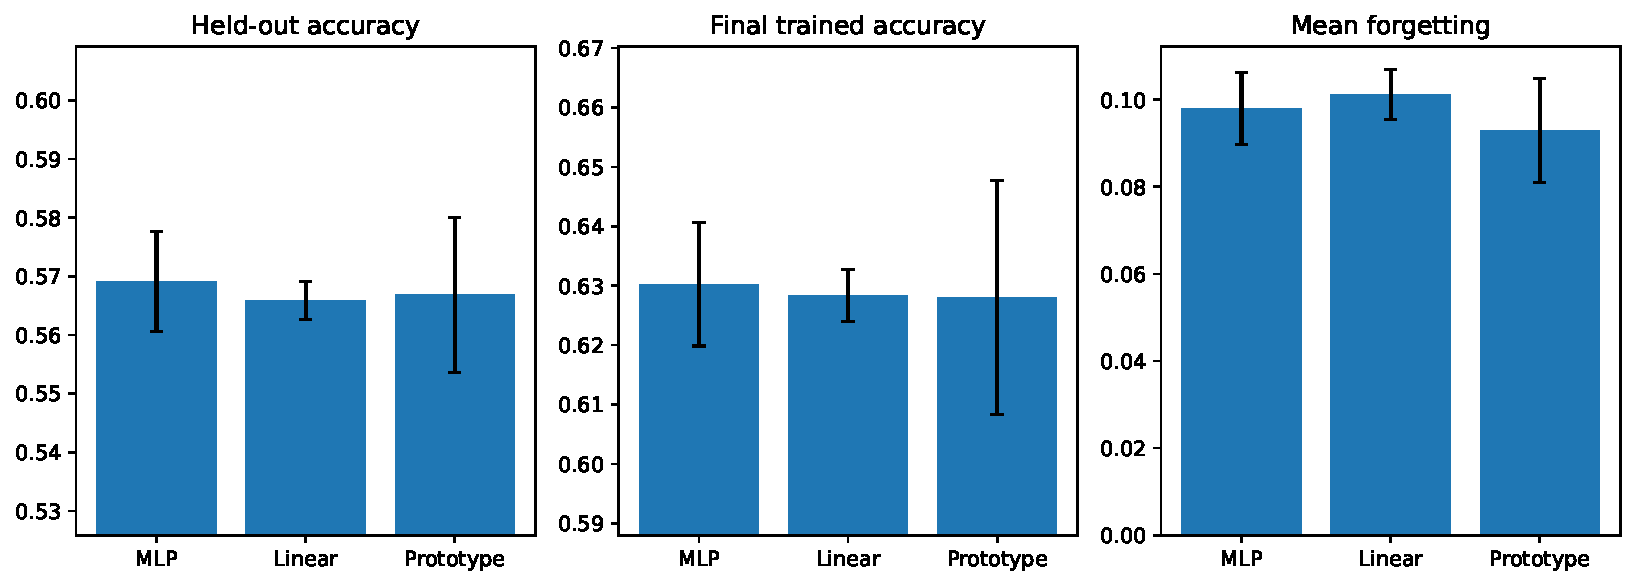
\includegraphics[width=.98\textwidth]{figures/operational_summary.pdf}
\caption{Held-out accuracy, final trained-angle accuracy, and forgetting. The methods are operationally similar within the declared pilot margin.}
\end{figure}
No routing architecture improves prediction or retention with a seed interval excluding zero. The non-degradation gate passes as an equivalence statement, not as superiority.

\section{Reviewer interpretation}
\subsection{What is now supported}
\begin{itemize}
\item v1.0.9: replicated candidate context geometry and held-out-source factor information;
\item v1.1.0: partial structural context-to-route mediation;
\item prototype routing: reproducible nominal order and trained-factor functional order over the MLP;
\item linear routing: a simpler mechanism that is at least as competitive and more promising causally;
\item no material operational degradation under matched compute.
\end{itemize}

\subsection{What is not supported}
\begin{itemize}
\item held-out functional mediation;
\item prototype causal specificity;
\item prediction-identity preservation under prototype interventions;
\item stable functional host specialization;
\item memory transport;
\item accuracy, forgetting, robustness, or cost superiority;
\item a Riemannian-manifold claim;
\item a full multi-objective energy-guided or RL controller;
\item any quantum advantage.
\end{itemize}

\subsection{Two methodological limitations that v1.1.1 must fix}
\subsubsection{The primary functional gate used trained factors}
The current functional candidate gate passes on the trained partition, while the held-out functional interval includes zero. The next primary gate must be held-out functional mediation.

\subsubsection{The functional cost matrix is method specific}
Each treatment trains its own hosts and then estimates a separate cost matrix $C^{(R_0)},C^{(R_1)},C^{(R_2)}$. A cross-method functional distance comparison therefore mixes route movement with changes in the host functions themselves. v1.1.1 must use a common frozen host bank and common primary matrix $C^\star$. Method-specific matrices may remain as secondary ecology measures.

\section{Complete v1.1.1 design: local stability and bridge isolation}
\subsection{Research question}
\begin{plainbox}[Primary question]
When the context representation, host bank, classifier, and host-function metric are all frozen and shared, which routing architecture most faithfully and stably transmits context geometry into functionally meaningful route changes on unseen factors and perturbations?
\end{plainbox}

\subsection{Frozen common objects}
For each seed, v1.1.1 should freeze:
\begin{equation}
P,\quad C_\phi,\quad \{g_h\}_{h=1}^{H},\quad Q,\quad C^\star,
\end{equation}
where $P$ is the sensory encoder, $C_\phi$ the aligned context encoder, $g_h$ the common host bank, $Q$ the classifier/synthesis map, and $C^\star$ the common functional host-cost matrix.

This design isolates $R_\theta$ rather than allowing host function and route geometry to co-adapt.

\subsection{Four routers}
\begin{enumerate}
\item R0: flexible MLP control;
\item R1: low-capacity linear router;
\item R2: prototype-energy router;
\item R3: hybrid directional-prototype energy.
\end{enumerate}
The hybrid is preregistered as
\begin{equation}
E_h(c)=\alpha\frac{d_C(c,\mu_h)^2}{2\sigma_h^2}-\beta a_h^\top c+b_h,
\qquad
r_h(c)=\frac{e^{-E_h(c)/\tau}}{\sum_k e^{-E_k(c)/\tau}}.
\end{equation}
The prototype term creates local territories; the directional term can preserve the global direction that the linear router transmitted well.

\subsection{Local continuity distribution}
For nearby empirical states $\mu_1,\mu_2$, measure
\begin{equation}
L_{\mathrm{local}}(\mu_1,\mu_2)=
\frac{d_H(R(\mu_1),R(\mu_2))}{d_{ZM}(\mu_1,\mu_2)+\varepsilon}.
\end{equation}
Report the full distribution, quantiles, tails, and neighborhood-conditional values, not only the mean. A router may have acceptable average sensitivity while containing rare discontinuities that destroy robustness.

\subsection{Perturbation suite}
The primary v1.1.1 suite should include:
\begin{itemize}
\item latent/context noise at matched norms;
\item factor-tangent and orthogonal perturbations;
\item ambiguous mixtures between adjacent contexts;
\item progressive drift along and away from the factor trajectory;
\item partial sensory corruption;
\item host-candidate permutation with index-equivariance checks;
\item route swaps between nearby and distant contexts;
\item host deletion and renormalization.
\end{itemize}
Memory deletion and inference-order perturbation should be activated when the explicit memory state enters the experiment.

\subsection{Metrics}
Compare Euclidean simplex distance, root-chord/Hellinger, Jensen--Shannon, Fisher--Rao-compatible measures, and functional Wasserstein/Sinkhorn distance. Retain a metric only if it improves route prediction, stability discrimination, drift detection, host specialization evidence, or controller auditability.

Mandatory outputs include route entropy, host dominance, route-switch rate, host contribution gain, ablation impact, route-swap impact, representation separation, route-function stability, cross-seed agreement, local sensitivity maps, and prediction-identity preservation.

\subsection{Primary gates}
\begin{enumerate}
\item held-out functional route-order effect has seed CI lower bound $>0$;
\item at least 80\% of seeds favorable;
\item local-continuity tail risk below preregistered threshold;
\item tangent functional CSR lower bound $>1$ in at least four of five seeds and mean CSR $>1.5$;
\item prediction-identity preservation lower bound $\ge0.95$;
\item route-swap effects are larger for distant than neighboring factor contexts;
\item no operational degradation beyond the declared equivalence margin.
\end{enumerate}
Ten-seed qualification should occur only after these five-seed mechanism gates pass.

\section{Subsequent Geometry-MMALS versions}
\subsection{v1.1.2: SPD covariance geometry and drift}
Representation and activation covariances are symmetric positive-definite objects. Compare:
\begin{align}
d_E(A,B)&=\norm{A-B}_F,\\
d_{LE}(A,B)&=\norm{\log A-\log B}_F,\\
d_{AI}(A,B)&=\norm{\log(A^{-1/2}BA^{-1/2})}_F.
\end{align}
Log-Euclidean and affine-invariant SPD geometry \cite{bhatia2007positive,pennec2006riemannian} should be retained only if they improve context separation, route prediction, stability, drift detection, or host specialization over Euclidean covariance controls.

\subsection{v1.1.3: route-function memory and transport}
Track route-function relations through continual stages. Required evidence includes old-region drift, path reconstruction, neighborhood retention, route-function stability, memory-deletion sensitivity, and comparison with no-transport and replay controls. The term \emph{parallel transport} is prohibited unless a suitable connection and geometric structure are explicitly defined and tested.

\subsection{v1.1.4: causal host specialization qualification}
Qualify host roles using multiple evidence families:
\begin{itemize}
\item non-trivial route entropy and host dominance patterns;
\item positive local host contribution gain;
\item localized ablation impact;
\item route-swap impact;
\item representation and gradient/contribution separation;
\item route-function stability through continual stages;
\item cross-seed role reproducibility after optimal matching.
\end{itemize}
Hub-and-partner ecologies are permitted. Raw route dominance is insufficient.

\section{From G1 geometry to G2 Energy-Guided routing}
The prototype router is not a competitor to the broader energy-guided design; it is a candidate geometric energy term:
\begin{equation}
E_h=\alpha E_h^{\mathrm{geo}}+\beta E_h^{\mathrm{host}}+
\gamma E_h^{\mathrm{memory}}+\delta E_h^{\mathrm{cost}}+
\eta E_h^{\mathrm{stability}}+\zeta E_h^{\mathrm{goal}}.
\end{equation}
v1.1.x should establish $E_h^{\mathrm{geo}}$ and its route-function consequences. G2 then adds uncertainty, saturation, cost, memory risk, stability, bottom-up host feedback, and goals. TPUT adds future prediction, regret, and goal-conditioned policy adaptation.

\begin{figure}[H]\centering
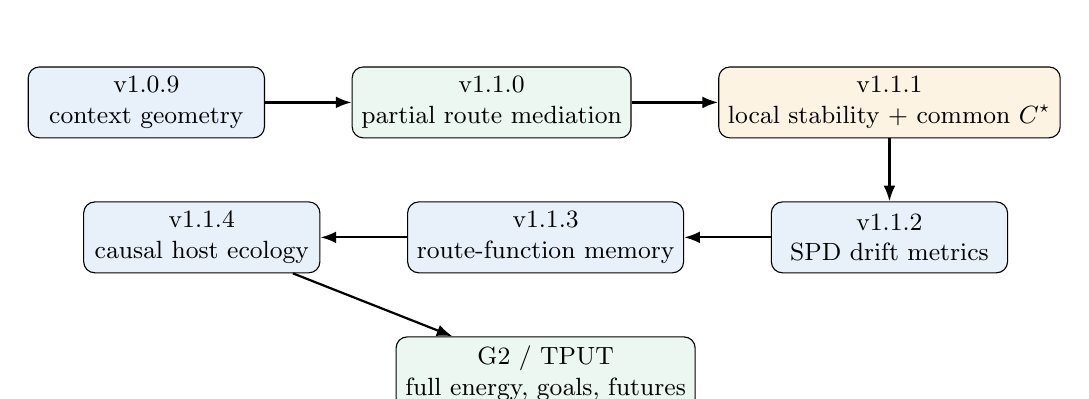
\begin{tikzpicture}[node distance=8mm and 11mm, every node/.style={font=\small}, box/.style={draw,rounded corners,align=center,minimum width=3cm,minimum height=.9cm,fill=softblue}, arr/.style={-{Latex[length=2mm]},thick}]
\node[box] (a) {v1.0.9\\context geometry};
\node[box,right=of a,fill=softgreen] (b) {v1.1.0\\partial route mediation};
\node[box,right=of b,fill=softorange] (c) {v1.1.1\\local stability + common $C^\star$};
\node[box,below=of c] (d) {v1.1.2\\SPD drift metrics};
\node[box,left=of d] (e) {v1.1.3\\route-function memory};
\node[box,left=of e] (f) {v1.1.4\\causal host ecology};
\node[box,below=of e,fill=softgreen] (g) {G2 / TPUT\\full energy, goals, futures};
\draw[arr] (a)--(b);\draw[arr] (b)--(c);\draw[arr] (c)--(d);\draw[arr] (d)--(e);\draw[arr] (e)--(f);\draw[arr] (f)--(g);
\end{tikzpicture}
\caption{Recommended progression. Each stage adds one falsifiable capability rather than a monolithic ecosystem redesign.}
\end{figure}

\section{Mandatory metric, protocol, and claim verification}
\subsection{Independent verification architecture}
\begin{equation*}
\text{Experiment outputs}\to\text{Metric Evaluator}\to\text{Protocol Verifier}\to\text{Claim Verifier}\to\text{Evidence Bundle}.
\end{equation*}
Every claim should emit one of \texttt{PASS}, \texttt{PARTIAL}, \texttt{FAIL}, or \texttt{NOT\_TESTED}.

\subsection{v1.1.0 machine-readable status}
\begin{table}[H]\centering\small
\caption{Verification interpretation of v1.1.0.}
\begin{tabularx}{\textwidth}{lclY}
\toprule
Claim & Status & Evidence & Reviewer interpretation\\
\midrule
Protocol integrity & PASS & frozen context, matched compute & clean five-seed pilot\\
Nominal route mediation & PARTIAL & trained and held-out positive intervals & candidate structural bridge\\
Functional route mediation & PARTIAL & trained positive, held-out null & not generalized\\
Causal specificity & FAIL & prototype CSR/DMR below gate & mechanism incomplete\\
Host ecology & FAIL & territories without stable ablation locality & roles unqualified\\
Operational non-degradation & PASS & within equivalence margin & not superiority\\
Memory transport & NOT\_TESTED & not implemented & future v1.1.3\\
Operational superiority & NOT\_TESTED & not primary and no positive interval & prohibited claim\\
\bottomrule
\end{tabularx}
\end{table}

\subsection{Red-team requirements}
The verifier must reject experiments with test leakage, hidden task identifiers, missing seeds, absent checkpoints, incomparable budgets, synthetic traces presented as real training, specialization claims without ablations, backward-transfer claims inferred from low forgetting, or route changes without target-objective improvement.

\subsection{Merge rule}
A geometric idea should be merged only if removing it makes the system objectively less performant, stable, compact, explainable, auditable, or verifiable. A sophisticated metric or visualization alone is not sufficient.

\section{Conclusion}
Geometry-MMALS has now crossed two distinct thresholds. v1.0.9 showed that a grounded context geometry can be learned and replicated. v1.1.0 shows that simple routing architectures can preserve more of that order than a flexible MLP. The bridge is nevertheless incomplete: functional geometry does not generalize to unseen factors, prototype interventions are not causally specific, route territories are not yet stable competencies, and no operational advantage appears.

The most informative next experiment is not a larger qualification run. It is v1.1.1: freeze the host functions, use a common functional metric, compare linear, prototype, and hybrid directional-prototype routing, and measure local stability and perturbation tails on held-out factors. This keeps the program understandable, reviewer-defensible, and cumulative.

\appendix
\section{Candidate claims in reviewer-safe language}
\begin{plainbox}[Recommended statement]
Across five matched-compute model seeds, freezing the replicated v1.0.9 context and replacing an unconstrained MLP router with low-capacity linear or prototype-energy routing increases the preservation of rotation-factor order in the route distribution. Prototype-energy routing yields replicated nominal order improvements on trained and held-out angles and a trained-factor improvement under a functional optimal-transport route metric. The functional effect does not generalize to held-out angles, and causal host specialization or operational benefit is not established.
\end{plainbox}

\section{Reproducibility and archive map}
The release includes the executable notebook, complete per-seed results, CSV aggregates, context and initialization hashes, source partition hashes, environment information, the 67-page execution PDF, the article and reviewer LaTeX sources, machine-readable verification rules, and SHA-256 checksums. The execution archive contains full notebook output and is distinct from the clean GitHub package.

\printbibliography
\end{document}
